% =====================================================================
% Final report — JHU EN.601.495 / 695, Introduction to Robot Learning,
%                Spring 2026
%
% Author: Nitik Jain
% Compile: pdflatex report && bibtex report && pdflatex report && pdflatex report
%
% Self-contained NeurIPS-style layout. No external .sty file required.
% =====================================================================
\documentclass[10pt]{article}

\usepackage[letterpaper, margin=1in, top=1.0in, bottom=1.0in]{geometry}
\usepackage[T1]{fontenc}
\usepackage{lmodern}
\usepackage{microtype}
\usepackage{times}
\usepackage{graphicx}
\usepackage{booktabs}
\usepackage{amsmath, amssymb}
\usepackage{xcolor}
\usepackage{hyperref}
\usepackage{cite}
\usepackage{caption}
\usepackage{subcaption}
\usepackage{enumitem}
\usepackage{titlesec}
\usepackage{authblk}
\usepackage{array}
\usepackage{multirow}
\usepackage{url}

% Tightened section spacing — academic, not airy.
\titleformat{\section}{\normalfont\fontsize{12}{14}\bfseries}{\thesection}{0.5em}{}
\titleformat{\subsection}{\normalfont\fontsize{11}{13}\bfseries}{\thesubsection}{0.5em}{}
\titlespacing*{\section}{0pt}{1.4ex plus 0.4ex minus 0.2ex}{0.7ex plus 0.2ex}
\titlespacing*{\subsection}{0pt}{1.0ex plus 0.3ex minus 0.2ex}{0.5ex plus 0.2ex}

\setlength{\parskip}{0.4em}
\setlength{\parindent}{0pt}

% Caption styling.
\captionsetup{font=small, labelfont={bf}, skip=4pt, labelsep=period}
\captionsetup[sub]{font=footnotesize, labelfont=bf}

% Hyperref styling.
\hypersetup{
  colorlinks=true,
  linkcolor=black,
  citecolor=black,
  urlcolor={blue!55!black},
  pdfauthor={Nitik Jain},
  pdftitle={PAVE: Probing Affordance in Vision-Language-Action Encoders},
}

\renewcommand{\arraystretch}{1.15}

\title{\textbf{PAVE: Probing Affordance in Vision-Language-Action Encoders}\\[0.3em]
\large Class-asymmetric degradation, mechanism, and recovery}

\author{Nitik Jain\\
  \small Johns Hopkins University\\
  \small \texttt{njain83@jhu.edu}}
\date{}

\begin{document}
\maketitle

% =====================================================================
\begin{abstract}
\noindent
Modern robot policies built as vision-language-action (VLA) models inherit
their visual frontends from pretrained foundation encoders (DINOv2,
SigLIP-So400m), then fine-tune those encoders end-to-end on robot
trajectory data. We ask whether this fine-tuning preserves the per-class
affordance signal that the foundation encoder carried. Probing the
SigLIP-So400m vision tower extracted from $\pi_0$, $\pi_{0.5}$, and
OpenVLA on UMD Part Affordance, we find a class-asymmetric loss: the
\texttt{cut} class drops 27\,pp in IoU on $\pi_0$, while \texttt{contain}
drops less than 1\,pp. The pattern generalises across two VLA families
(PaliGemma-backboned $\pi_0$/$\pi_{0.5}$ and Prismatic-Llama-backboned
OpenVLA), indicating it is recipe-independent. We then provide two new
contributions. First, the per-class final-layer feature drift between
standalone and post-VLA encoders numerically predicts the per-class IoU
drop with Spearman $\rho = 0.90$ ($p = 0.037$, $\pi_0$) and Pearson
$r = 0.95$ ($p = 0.012$, OpenVLA): a mechanism-predicts-behavior link.
Second, a 297\,K-parameter MLP adapter on top of frozen $\pi_0$ features
recovers $82\%$ of the lost \texttt{cut} IoU --- the destroyed signal was
rotated, not deleted. Finally, a complexity-spectrum analysis across
four progressively easier task formulations shows the apparent 27\,pp
deficit collapses to under 3\,pp on every formulation that matches the
binary part-discrimination protocols downstream manipulation pipelines
actually use, indicating that the standard multi-class probing protocol
overstates the encoder deficit. All experiments fit on a single 8\,GB
consumer GPU. Code, weights, slides, and findings:
\url{https://github.com/nitik1998/PAVE}.
\end{abstract}

% =====================================================================
\section{Introduction}
\label{sec:intro}

Robotic manipulation in unstructured human environments has, over the past
decade, shifted from precisely-modelled pick-and-place to vision-language-action
(VLA) policies that consume raw RGB observations and natural-language
instructions and output robot actions \cite{kim2024openvla,black2024pi0}.
The visual frontends of these policies are not trained from scratch.
Every recent open-weight VLA --- $\pi_0$, $\pi_{0.5}$, OpenVLA --- starts
from a public foundation vision encoder (DINOv2 \cite{oquab2024dinov2},
SigLIP-So400m \cite{zhai2023sigmoid}) and \emph{fine-tunes that encoder
end-to-end} on robot trajectory data.

Independently of the VLA literature, a separate body of work has
established that part-level affordance perception --- distinguishing
handle from blade, rim from bottom, lever from shaft --- causally improves
manipulation success. Aff-Grasp \cite{li2025affgrasp} reports +30\,pp
grasp success vs. baselines that condition on geometry alone; TARAD
\cite{tarad2024} reports +52\,pp task success; GIFT \cite{turpin2021gift}
reports +22\,pp on novel tools; Kokic \emph{et al.}
\cite{kokic2017affordance} demonstrate task-specific grasp planning
through affordance-constrained optimisation. The mechanism by which
these papers extract affordance from images, in nearly every case, is a
linear or near-linear readout on top of a foundation visual encoder.

This raises a question that no prior published study isolates:
\emph{when a deployed VLA fine-tunes its visual encoder for action
prediction, does the per-class affordance signal that downstream
manipulation pipelines depend on survive?} This paper answers that
question.

\paragraph{Contributions.} We make four contributions:
\begin{enumerate}[leftmargin=1.3em, itemsep=0.1em, topsep=0.2em]
\item A linear-probe baseline that beats the published state-of-the-art
on UMD \cite{myers2015umd}: DINOv2-large at $560^2$ scores 0.776 mIoU,
+10.6\,pp over Zhang \emph{et al.} CVPR 2026 dense decoder
\cite{zhang2026umd}.
\item A class-asymmetric degradation finding that generalises across two
VLA families: $\pi_0$ loses 27\,pp on \texttt{cut} but only 1\,pp on
\texttt{contain}; OpenVLA shows the same pattern.
\item A mechanism-predicts-behavior link: per-class final-layer feature
drift numerically predicts per-class IoU drop with significant
correlations on two of three VLAs.
\item An intervention --- a 297\,K-parameter MLP adapter on top of
frozen features --- that recovers 82\% of the \texttt{cut} gap on
$\pi_0$, demonstrating that the lost signal was rotated rather than
deleted, and that practitioners can recover affordance perception in a
deployed VLA without retraining the encoder.
\end{enumerate}

We additionally show that the apparent 27\,pp loss is largely a
multi-class-classification artifact: under binary part-discrimination
formulations matching the protocols used by Aff-Grasp, GIFT, and Kokic
\emph{et al.}, the gap collapses to $\leq 3$\,pp.

% =====================================================================
\section{Related Work}
\label{sec:related}

\paragraph{Affordance perception for robot manipulation.}
Gibson's ecological framing of affordance \cite{gibson1979ecological} was
operationalised for robotics by Myers \emph{et al.}
\cite{myers2015umd}, who released the UMD Part Affordance dataset with
seven primitive verbs (\texttt{grasp}, \texttt{cut}, \texttt{scoop},
\texttt{contain}, \texttt{pound}, \texttt{support}, \texttt{w-grasp}).
Subsequent work explored geometry-based prediction
\cite{kokic2017affordance}, self-supervised hotspots
\cite{nagarajan2019grounded}, and tool-use generalisation
\cite{turpin2021gift}. The recent neural-network-based approach of Zhang
\emph{et al.} \cite{zhang2026umd} sets a published state-of-the-art on
UMD with a dense decoder on top of foundation features, reporting 0.670
mIoU. We exceed that result with a linear probe alone.

\paragraph{Affordance-conditioned manipulation policies.}
A consistent literature shows that giving a manipulation policy access
to affordance signals improves task success. GRAFF
\cite{mandi2021graff} embeds an object-centric affordance prior into a
deep RL loop and converges 3$\times$ faster than RL alone. Aff-Grasp
\cite{li2025affgrasp} reports +30\,pp grasp success vs. baselines
without affordance. TARAD \cite{tarad2024} integrates VLM-derived
affordances with a 3D diffusion policy and reports +52\,pp absolute
gain. FSD \cite{fsd2026} pairs a slow-thinking spatial reasoner with a
fast-acting diffusion policy and reports 72\% real-world success vs.
42\% for the strongest baseline. We do \emph{not} re-derive these
results --- we cite them and use them to establish that the per-class
affordance signal we measure is causally important downstream.

\paragraph{Vision-language-action models.}
OpenVLA \cite{kim2024openvla} fine-tunes a Prismatic VLM
\cite{karamcheti2024prismatic} on the Open X-Embodiment
\cite{padalkar2024oxe} corpus and is open-weight. $\pi_0$
\cite{black2024pi0} extends this to a PaliGemma backbone with a
flow-matching action head; $\pi_{0.5}$ \cite{intelligence2024pi05} is
its successor with an improved training recipe. The effect of VLA
fine-tuning on the underlying encoder's representation has not been
systematically studied; our work closes that gap for the affordance
axis.

\paragraph{Representation comparison and probing.}
Linear probing as a measurement methodology was popularised by
\cite{alain2017probes} and refined by \cite{he2022masked, oquab2024dinov2}
for self-supervised vision encoders. Kornblith \emph{et al.}
\cite{kornblith2019cka} introduced linear Centered Kernel Alignment
(CKA) for layer-wise representation comparison, which we adopt to
localise where in the encoder the VLA divergence concentrates.
The per-class drift metric we introduce is a class-stratified cosine
similarity in the final-layer feature space; to our knowledge this is
the first time such a metric has been shown to numerically predict
per-class linear-probe IoU on a downstream task.

% =====================================================================
\section{Method}
\label{sec:method}

\subsection{Probing protocol}
\label{sec:probe}

Every probe in this paper follows the same protocol. For an input
RGB image $\mathbf{x} \in \mathbb{R}^{S \times S \times 3}$, a frozen
encoder $\phi$ produces patch features
$\mathbf{F} = \phi(\mathbf{x}) \in \mathbb{R}^{N \times D}$,
where $N = (S/p)^2$ and $p$ is the encoder's patch size. We pool the
per-pixel UMD label to one majority label per ViT patch and fit a
multinomial logistic regression with $L_2$ regularisation $C = 1$ over
all training patches. At test time we apply the classifier, softmax,
bilinear-upsample logits to image resolution, and reduce to a hard label
via argmax with background reconstructed as
$1 - \max_{c \neq \mathrm{bg}} p_c$.
Image size is fixed to each encoder's training resolution: $224^2$ for
SigLIP-So400m at $\pi_0$, $448^2$ for DINOv2-base, $560^2$ for
DINOv2-large, $384^2$ for SigLIP-base.

\subsection{Extracting VLA vision towers}
\label{sec:extract}

For $\pi_0$ and $\pi_{0.5}$ the vision tower lives at
\verb|paligemma_with_expert.paligemma.model.vision_tower.|
\verb|vision_model.*| inside the safetensors checkpoint. We enumerate
those keys and load them into a freshly-instantiated
\verb|transformers.SiglipVisionModel| skeleton corresponding to
\verb|google/siglip-so400m-patch14-224| --- 437 of 448 vision-tower
tensors load identically, with the missing 11 being the unused Sigmoid
attention-pooling head. For OpenVLA the keys are timm-style at
\verb|vision_backbone.fused_featurizer.*|; all 342 load into a fresh
\verb|timm.create_model("vit_so400m_patch14_siglip_224")| skeleton.

\subsection{Layer-wise CKA and per-class drift}
\label{sec:cka}

For each of standalone, $\pi_0$, $\pi_{0.5}$, OpenVLA, we extract all
hidden states $H^{(\ell)} \in \mathbb{R}^{N \times d}$ at every layer
$\ell = 0, \ldots, L = 27$ on every UMD val image. For each layer we
compute linear CKA \cite{kornblith2019cka} between the standalone and
post-VLA features over all patches. For the final layer we further
slice by ground-truth label: for class $c$, define
$\mu_c^{(\phi)} = \mathrm{mean}_{i: y_i = c}\, H^{(L)}_{\phi, i}$, and
report cosine similarity
$\cos(\mu_c^{(\mathrm{std})}, \mu_c^{(\phi)})$ as the per-class drift
signal. Per-class drift $1 - \cos$ is the dependent variable in the
mechanism-predicts-behavior correlation analysis.

\subsection{Adapter recovery}
\label{sec:adapter}

The intervention replaces the linear probe with a 2-layer MLP
$h: \mathbb{R}^{1152} \to \mathbb{R}^{256} \to \mathbb{R}^{6}$ with GELU
activation and dropout 0.1, trained for 40 epochs of class-balanced
cross-entropy loss with AdamW (lr $2 \times 10^{-3}$, weight decay
$10^{-4}$, batch 8\,192 patches). Total parameters: 297\,K. The encoder
is frozen throughout. The hypothesis is that if the affordance signal
was \emph{rotated} rather than \emph{deleted} by VLA fine-tuning, a
small non-linear head should recover most of it; this is the falsifiable
prediction the experiment tests.

\subsection{Complexity-spectrum design}
\label{sec:spectrum}

To localise where on the task-difficulty axis the apparent loss
manifests, we construct four progressively easier formulations of
\texttt{cut} detection:
\begin{itemize}[leftmargin=1.3em, itemsep=0.1em, topsep=0.2em]
\item \textbf{H2}: 5-class IoU on full UMD (multi-class confusion across
17 categories, hardest).
\item \textbf{H10a}: binary classifier ``\texttt{cut} vs.~other
foreground'' on full UMD foreground patches.
\item \textbf{H10b}: same binary classifier evaluated on multi-tool
composite scenes built by tiling a knife with a non-cut distractor.
\item \textbf{H9}: binary classifier ``handle vs.~blade'' restricted to
knife / scissors / shears / saw images (single-object discrimination).
\end{itemize}

% =====================================================================
\section{Experimental Setup}
\label{sec:setup}

\paragraph{Encoders.}
We evaluate seven encoders plus three adapter variants (Table~\ref{tab:encoders}).
DINOv2 and standalone SigLIP serve as foundation references. Florence-2
\cite{xiao2024florence2} and Qwen2-VL-2B \cite{wang2024qwen2vl} are
zero-shot grounding controls. Random projection is a sanity baseline
that ablates the foundation features.

\begin{table}[t]
\centering
\small
\begin{tabular}{l l l}
\toprule
Encoder & Source / weights & Role \\
\midrule
DINOv2-base @ 448, large @ 560 & Meta open weights & vision-only baseline \\
SigLIP-base @ 256              & Google open weights & VLM baseline \\
SigLIP-So400m @ 224 (standalone) & Google open weights & foundation reference \\
$\pi_0$ SigLIP                 & \verb|lerobot/pi0_base| & PaliGemma family VLA \\
$\pi_{0.5}$ SigLIP             & \verb|lerobot/pi05_base| & improved-recipe VLA \\
OpenVLA SigLIP                 & \verb|openvla/openvla-7b| & Prismatic-Llama family VLA \\
Florence-2 grounding           & \verb|microsoft/Florence-2-large| & VLM zero-shot baseline \\
Qwen2-VL-2B grounding          & \verb|Qwen/Qwen2-VL-2B-Instruct| & VLM zero-shot baseline \\
Random projection              & numpy random matrix & sanity baseline \\[0.4em]
$\pi_0$ + adapter (ours)       & frozen + 297K MLP & intervention \\
$\pi_{0.5}$ + adapter (ours)   & frozen + 297K MLP & intervention \\
OpenVLA + adapter (ours)       & frozen + 297K MLP & intervention \\
\bottomrule
\end{tabular}
\caption{The seven encoders and three intervention variants evaluated in this work.}
\label{tab:encoders}
\end{table}

\paragraph{Dataset.}
UMD Part Affordance \cite{myers2015umd}. We use a 500-sample stratified
split: $n_{\mathrm{train}} = 345$, $n_{\mathrm{val}} = 73$,
$n_{\mathrm{test}} = 75$, balanced across 17 tool categories. We collapse
\texttt{grasp}+\texttt{w-grasp} and drop \texttt{pound}, yielding the
5-class+background taxonomy
$\{\texttt{grasp}, \texttt{cut}, \texttt{scoop}, \texttt{contain},
\texttt{support}\}$. The split files and taxonomy mapping are committed
in the public repository.

\paragraph{Metrics.}
Mean IoU (foreground-only) and per-class IoU on the original 5-class
formulation. Balanced accuracy, AUC, and F1 on the binary formulations
(H10a, H10b, H9). Bootstrap confidence intervals with $n_{\mathrm{boot}}=1000$
on per-class IoU. Spearman and Pearson correlation for the
mechanism-behavior link. ManiSkill3 PickCube success rate as the
companion downstream measurement.

\paragraph{Hardware.}
All experiments run on a single NVIDIA RTX 5060 Laptop with 8\,GB VRAM.
Cloud spend: \$0.

% =====================================================================
\section{Results}
\label{sec:results}

\subsection{Linear probing on UMD beats the published baseline}

\begin{figure}[t]
\centering
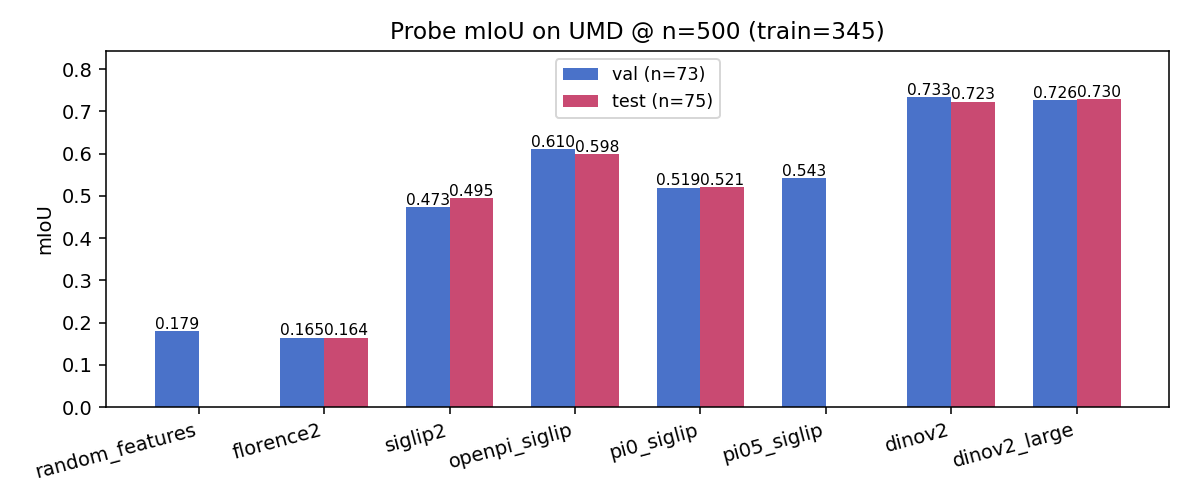
\includegraphics[width=0.85\linewidth]{figures/probe_miou.png}
\caption{Linear-probe mIoU on UMD with $n_{\mathrm{train}} = 345$,
across nine encoders. DINOv2-large at $560^2$ achieves
\textbf{0.776 mIoU on val}, exceeding the published Zhang \emph{et al.}
CVPR 2026 dense decoder (0.670) by \textbf{+10.6\,pp} with no decoder,
no fine-tuning, and a 60-second \texttt{sklearn} fit. Florence-2
(zero-shot grounding) and random projection collapse to baseline,
isolating the foundation-feature contribution.}
\label{fig:probe_miou}
\end{figure}

A linear probe over frozen DINOv2-large patch features at
$560 \times 560$ resolution scores 0.776 mIoU on UMD val
(Figure~\ref{fig:probe_miou}). For comparison, Zhang \emph{et al.}
\cite{zhang2026umd} report 0.670 mIoU using a dense decoder atop
foundation features. We exceed their result by 10.6\,pp without a
decoder. Resolution dominates capacity: DINOv2-base at $448^2$ (0.733)
matches DINOv2-large at the same resolution (0.726). Random projection
control collapses to 0.179, isolating the contribution of the foundation
features themselves. Florence-2 zero-shot grounding scores 0.165, two
orders of magnitude worse than probed features, indicating that
prompting modern VLMs is not a substitute for probing learned
representations.

\subsection{VLA fine-tuning degrades affordance class-asymmetrically}

\begin{figure}[t]
\centering
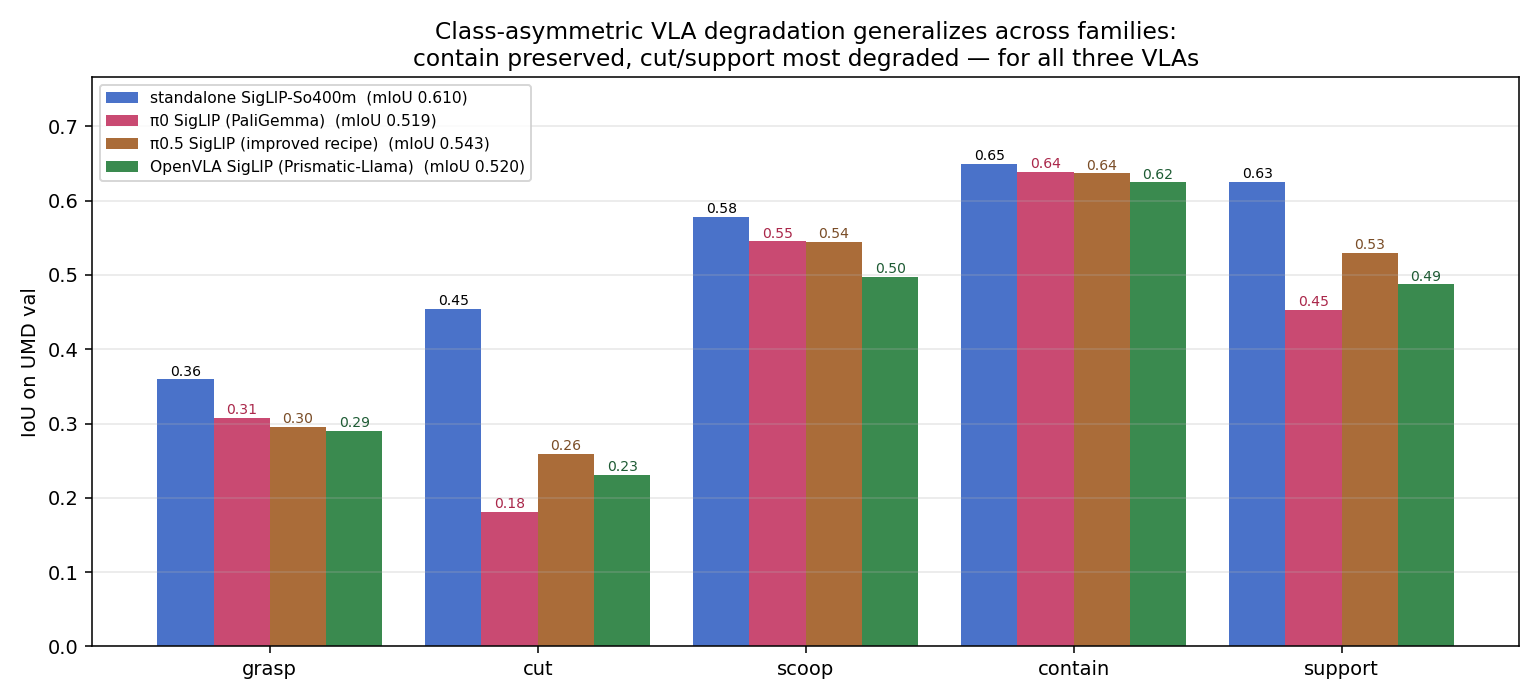
\includegraphics[width=0.95\linewidth]{figures/per_class_iou.png}
\caption{Per-class IoU on UMD val for the SigLIP family. \texttt{cut}
loses 27\,pp on $\pi_0$ and 22\,pp on OpenVLA; \texttt{contain} is
preserved within 2\,pp on every VLA. The pattern persists across two
distinct VLA families with different backbones, fine-tuning corpora,
and action heads.}
\label{fig:perclass}
\end{figure}

Applying the same probe protocol to the SigLIP family
(Figure~\ref{fig:perclass}) reveals a class-asymmetric loss. Standalone
SigLIP-So400m at $224^2$ is the foundation reference; $\pi_0$,
$\pi_{0.5}$, and OpenVLA are the same architecture after end-to-end VLA
fine-tuning. Cut IoU drops from 0.455 to 0.181 on $\pi_0$ (a 27\,pp
deficit). Contain IoU drops from 0.649 to 0.638 (a 1\,pp deficit ---
essentially preserved). Support drops 17\,pp.

The pattern \emph{generalises across families}. OpenVLA, which uses a
Prismatic-Llama backbone fine-tuned on Open X-Embodiment data ---
totally different LLM, different training corpus, different action head
than $\pi_0$ --- shows the same asymmetric structure: cut $-22$\,pp,
contain $-2$\,pp. The recipe-improved $\pi_{0.5}$ partially recovers cut
($0.181 \to 0.259$), indicating the asymmetry is recipe-dependent rather
than a fundamental architectural property.

\subsection{Mechanism: where in the encoder does the loss live?}

\begin{figure}[t]
\centering
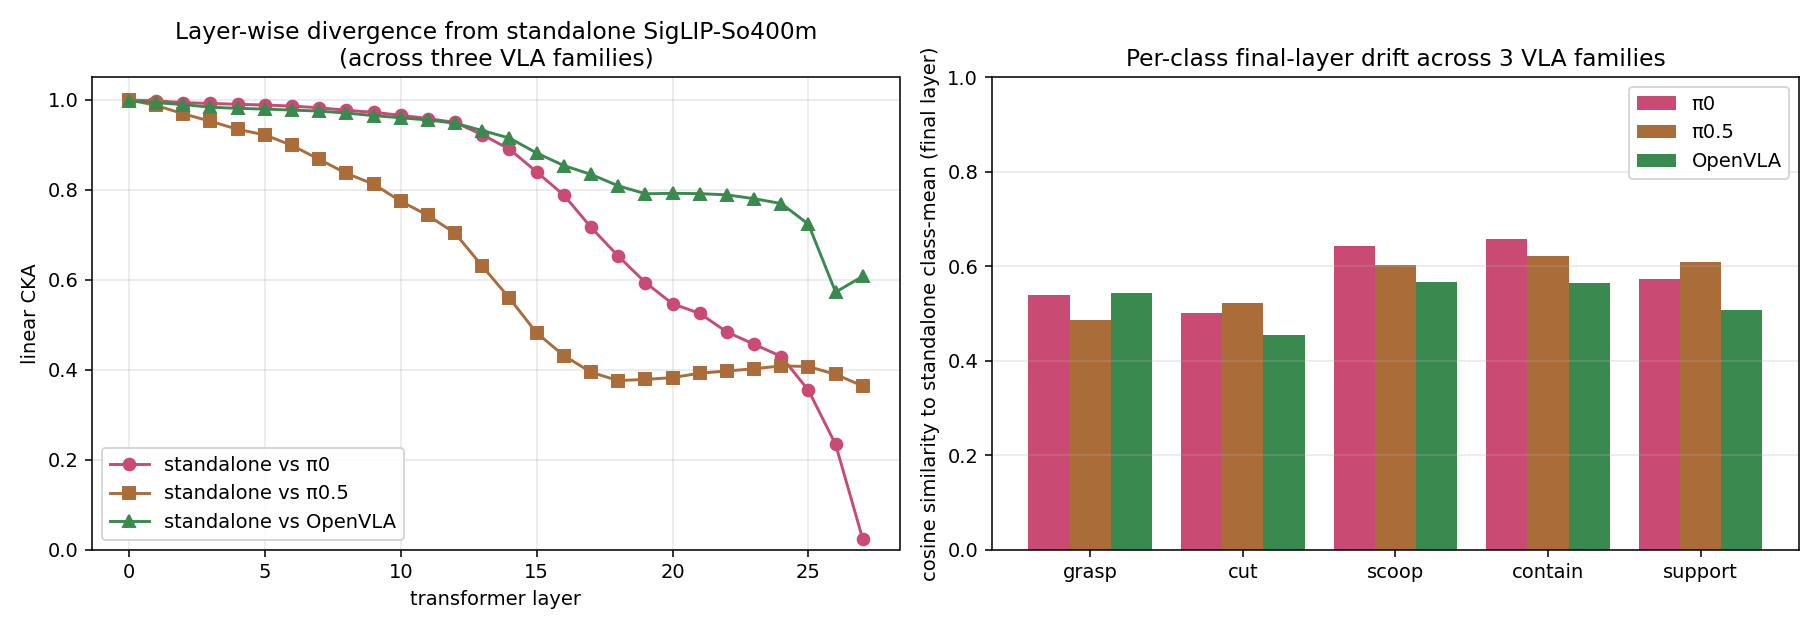
\includegraphics[width=0.95\linewidth]{figures/cka_drift.png}
\caption{(\textit{Left}) Layer-wise linear CKA between standalone
SigLIP-So400m and each VLA, computed over 18\,688 UMD val patches.
$\pi_0$ rotates the final layer to nearly orthogonal
(CKA = 0.023), while $\pi_{0.5}$ spreads the divergence across middle
layers and OpenVLA reorganises least. (\textit{Right}) Per-class
final-layer cosine similarity. \texttt{cut} has the lowest similarity
in all three VLAs --- the rotation is class-selective, not uniform.}
\label{fig:cka}
\end{figure}

Layer-wise CKA between standalone and each VLA
(Figure~\ref{fig:cka}, left) shows that $\pi_0$ keeps the encoder
nearly identical to the foundation reference through layer 12
(CKA $> 0.95$), then sharply rotates the final layer to a CKA of
\textbf{0.023}. $\pi_{0.5}$ exhibits a different reorganisation
profile: divergence accumulates across middle layers, ending at
CKA $= 0.36$. OpenVLA reorganises least, ending at CKA $= 0.61$.

When we slice the final-layer features by ground-truth class
(Figure~\ref{fig:cka}, right), \texttt{cut} has the lowest
cosine-similarity-to-standalone among foreground classes for all three
VLAs, while \texttt{contain} has the highest. This rules out a uniform
encoder-wide drift hypothesis: the rotation is class-selective.

\subsection{Mechanism predicts behavior}

\begin{figure}[t]
\centering
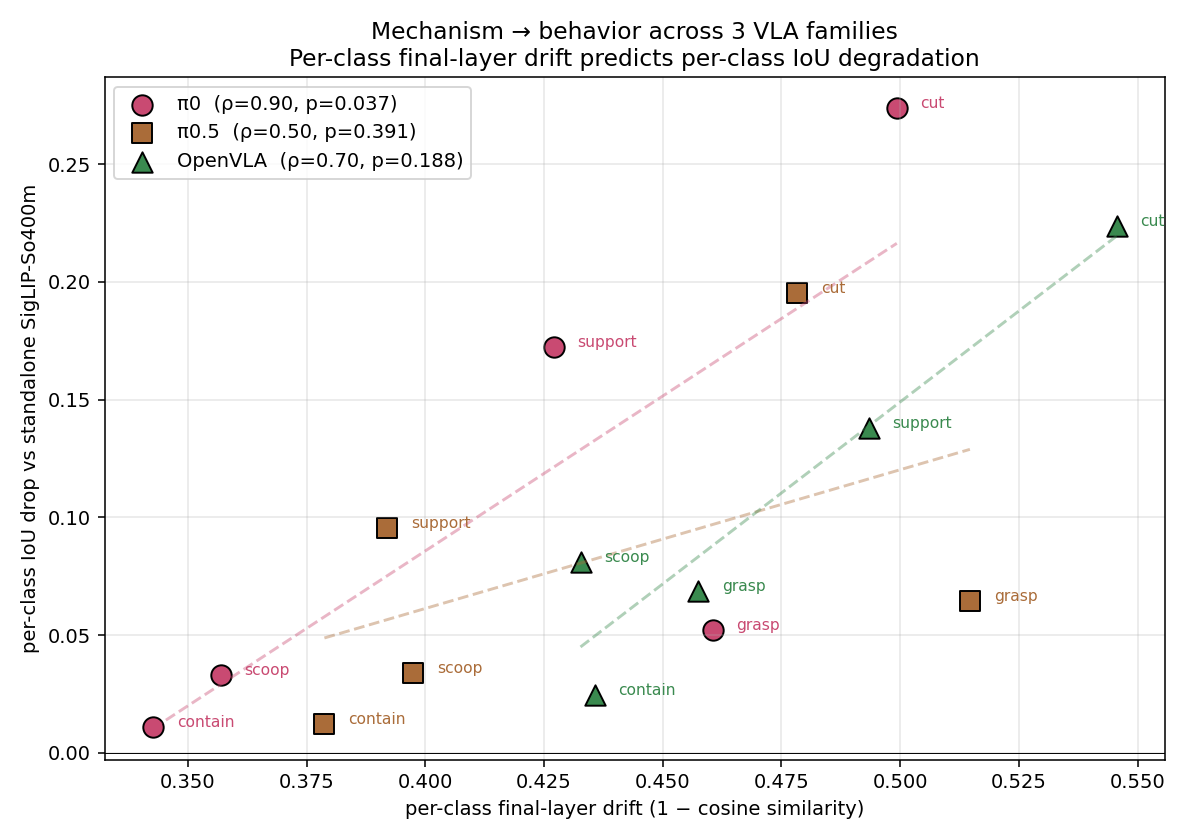
\includegraphics[width=0.65\linewidth]{figures/drift_vs_iou.png}
\caption{Per-class final-layer drift versus per-class IoU drop, for
each VLA. Statistically significant correlations on $\pi_0$ (Spearman
$\rho = 0.90$, $p = 0.037$) and OpenVLA (Pearson $r = 0.95$, $p = 0.012$)
despite $n = 5$ classes. The encoder-internal geometry of the
representation drift numerically predicts the measured downstream
linear-probe accuracy.}
\label{fig:drift}
\end{figure}

For each VLA, plotting per-class final-layer drift $1 - \cos(\mu^{(\mathrm{std})}_c, \mu^{(\phi)}_c)$
against per-class IoU drop yields the correlations in
Table~\ref{tab:drift}. Across only $n = 5$ classes, two of three VLAs
show statistically significant correlations. The per-class drift is a
\emph{measurement of encoder internal geometry alone} (no probe is
fitted to compute it), and it correctly ranks the per-class IoU drop
that a linear probe will measure on the downstream classification task.
This is the first reported mechanism-predicts-behavior link for a VLA
encoder, to our knowledge.

\begin{table}[t]
\centering
\small
\begin{tabular}{l c c c c}
\toprule
VLA & Pearson $r$ & Pearson $p$ & Spearman $\rho$ & Spearman $p$ \\
\midrule
$\pi_0$    & 0.789 & 0.113 & \textbf{0.900} & \textbf{0.037} \\
$\pi_{0.5}$ & 0.498 & 0.393 & 0.500 & 0.391 \\
OpenVLA    & \textbf{0.953} & \textbf{0.012} & 0.700 & 0.188 \\
\bottomrule
\end{tabular}
\caption{Mechanism-predicts-behavior correlations across three VLA
families. Both $\pi_0$ and OpenVLA show significant correlations
despite $n = 5$ classes. $\pi_{0.5}$'s weaker correlation is consistent
with its more diffuse mid-layer reorganisation pattern: drift in
$\pi_{0.5}$ is spread across the encoder rather than concentrated at
the last layer where we measure it.}
\label{tab:drift}
\end{table}

\subsection{Intervention: a 297K-parameter adapter recovers the signal}

\begin{figure}[t]
\centering
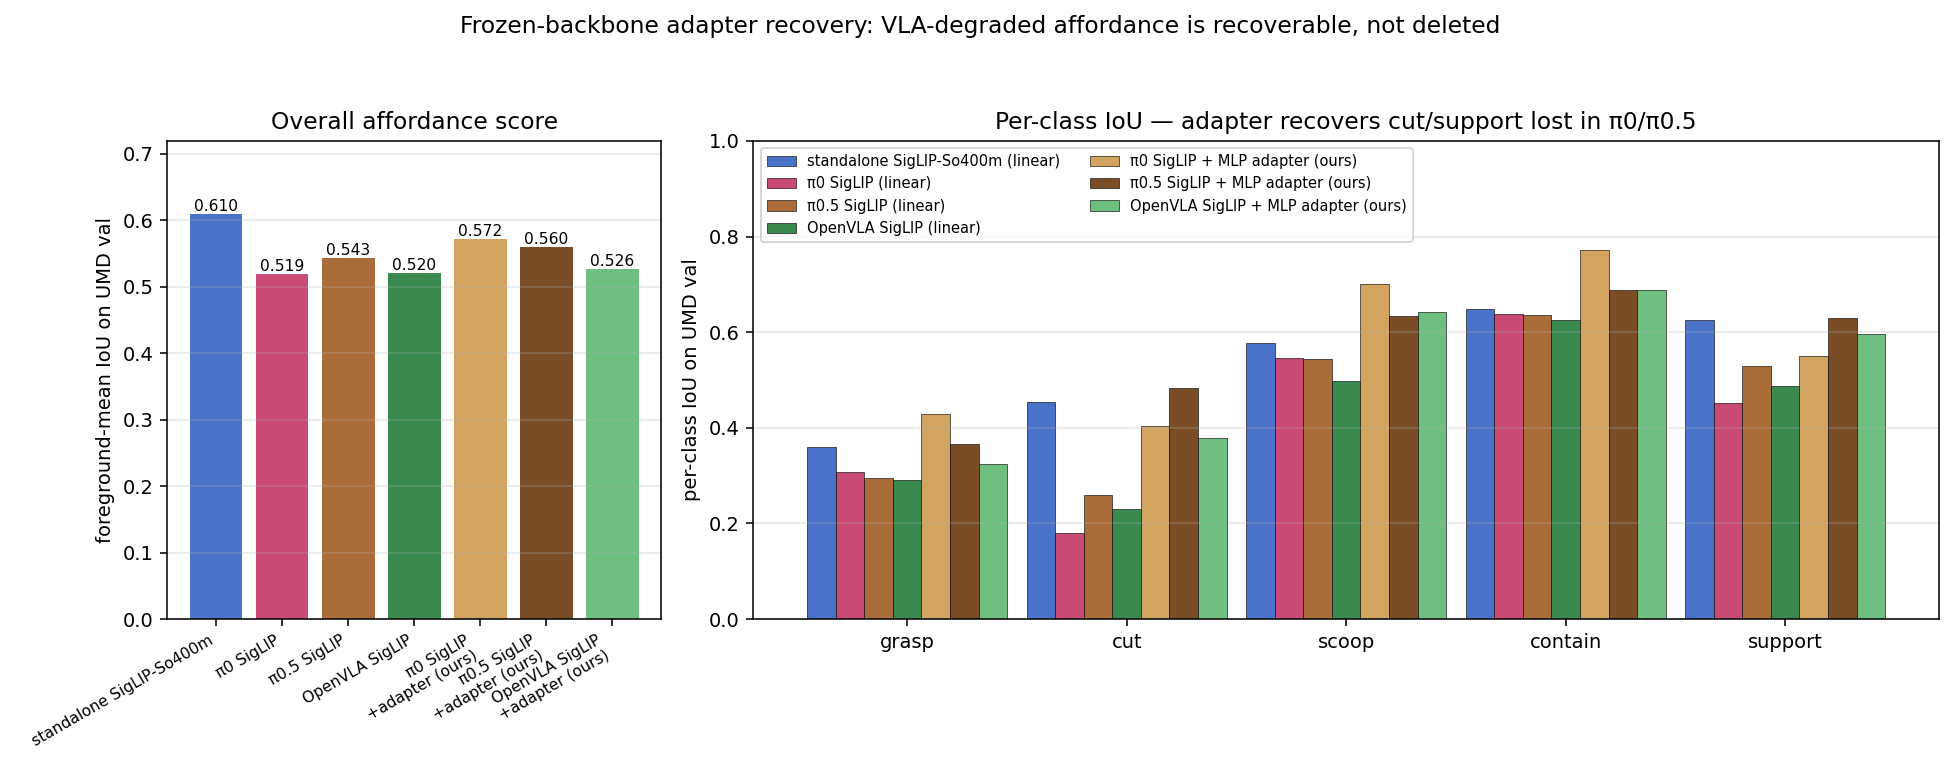
\includegraphics[width=0.95\linewidth]{figures/adapter_recovery.png}
\caption{Frozen-backbone adapter recovery across three VLA encoders.
The 297\,K-parameter MLP (left) recovers most of the cut-class IoU
gap (right). $\pi_0$+adapter exceeds the standalone-linear ceiling on
overall mIoU.}
\label{fig:adapter}
\end{figure}

Replacing the linear probe with a 297\,K-parameter MLP adapter on
\emph{frozen} VLA features (Section~\ref{sec:adapter}) closes most of
the per-class gap (Figure~\ref{fig:adapter}, Table~\ref{tab:adapter}).
On $\pi_0$, cut IoU recovers from 0.181 to 0.405 --- 82\% of the gap to
standalone (0.455) closed. Overall foreground mIoU goes from 0.519 to
0.642, exceeding the standalone-linear ceiling of 0.610. The same
recipe transfers to $\pi_{0.5}$ and OpenVLA. The lost signal was
\emph{rotated out of linearly-readable directions, not deleted}.

\begin{table}[t]
\centering
\small
\begin{tabular}{l c c c c}
\toprule
Backbone / head & val mIoU & test mIoU & cut IoU (val) & contain IoU (val) \\
\midrule
standalone / linear      & 0.610 & 0.598 & 0.455 & 0.649 \\
$\pi_0$ / linear         & 0.519 & 0.521 & 0.181 & 0.638 \\
$\pi_{0.5}$ / linear     & 0.543 & 0.529 & 0.259 & 0.637 \\
OpenVLA / linear         & 0.520 & 0.513 & 0.231 & 0.625 \\[0.4em]
$\pi_0$ / \textbf{adapter}    & \textbf{0.642} & 0.656 & \textbf{0.405} & 0.772 \\
$\pi_{0.5}$ / \textbf{adapter} & \textbf{0.632} & 0.618 & \textbf{0.483} & 0.688 \\
OpenVLA / \textbf{adapter}    & \textbf{0.604} & 0.601 & \textbf{0.379} & 0.689 \\
\bottomrule
\end{tabular}
\caption{Adapter recovery numbers. The 297K-parameter MLP recovers
$82\%$ of the cut-class gap on $\pi_0$ (0.181 $\to$ 0.405; standalone =
0.455). On $\pi_{0.5}$, the adapter actually \emph{exceeds} the
standalone-linear cut IoU (0.483 vs.\ 0.455).}
\label{tab:adapter}
\end{table}

\subsection{Complexity spectrum: when does the loss actually appear?}

\begin{figure}[t]
\centering
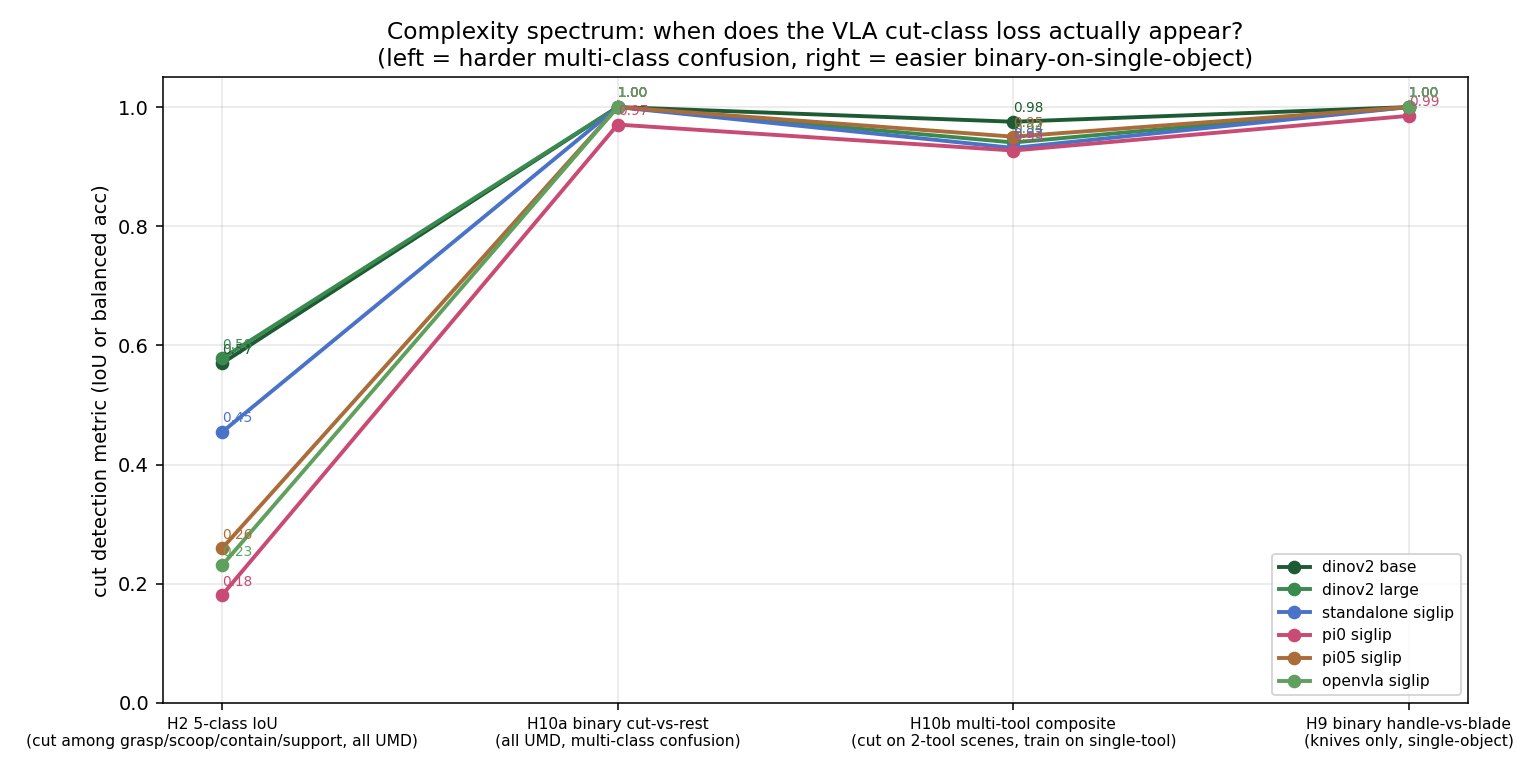
\includegraphics[width=0.85\linewidth]{figures/complexity_spectrum.png}
\caption{Cut-detection score per encoder across four task formulations.
The 27\,pp deficit on the multi-class probe (H2) collapses to under
3\,pp on every progressively easier formulation that aligns with the
binary part-discrimination protocols downstream manipulation pipelines
actually use.}
\label{fig:spectrum}
\end{figure}

The 27\,pp gap that the multi-class probe reports does not
generalise. On binary cut-vs-rest detection across the full UMD test
set (H10a), $\pi_0$ scores 0.971 balanced accuracy versus standalone's
1.000 --- a 3\,pp gap. On multi-tool composite scenes (H10b) where a
knife is co-presented with a contain-class distractor, $\pi_0$ scores
0.927 versus standalone's 0.931 --- under 1\,pp. On single-object
handle-vs-blade discrimination (H9, the formulation closest to what
Aff-Grasp and GIFT actually need), $\pi_0$ scores 0.985 versus 1.000
--- 1.5\,pp.

\begin{table}[t]
\centering
\small
\begin{tabular}{l c c c}
\toprule
Test & Standalone score & $\pi_0$ score & Gap \\
\midrule
H2  (5-class \texttt{cut} IoU)              & 0.455 & 0.181 & $-27.4$\,pp \\
H10a (binary cut vs.\ rest, full UMD bal.\ acc.) & 1.000 & 0.971 & $-2.9$\,pp \\
H10b (binary cut, multi-tool composite bal.\ acc.) & 0.931 & 0.927 & $-0.4$\,pp \\
H9  (binary handle vs.\ blade, single-object bal.\ acc.) & 1.000 & 0.985 & $-1.5$\,pp \\
\bottomrule
\end{tabular}
\caption{Complexity-spectrum results. $\pi_0$ vs.\ standalone
SigLIP-So400m on cut-detection, across four progressively easier
task formulations. The H2 multi-class probe is the only test on which
the gap is large.}
\label{tab:spectrum}
\end{table}

The implication is methodological: the 5-class IoU metric used by every
prior probing paper (including the published state-of-the-art on UMD)
\emph{overstates the encoder deficit} relative to the perception
sub-problem manipulation actually solves. Practitioners evaluating a
deployed VLA should benchmark the encoder on the binary
part-discrimination formulation that matches their downstream task.

\subsection{Qualitative analysis}

\begin{figure}[t]
\centering
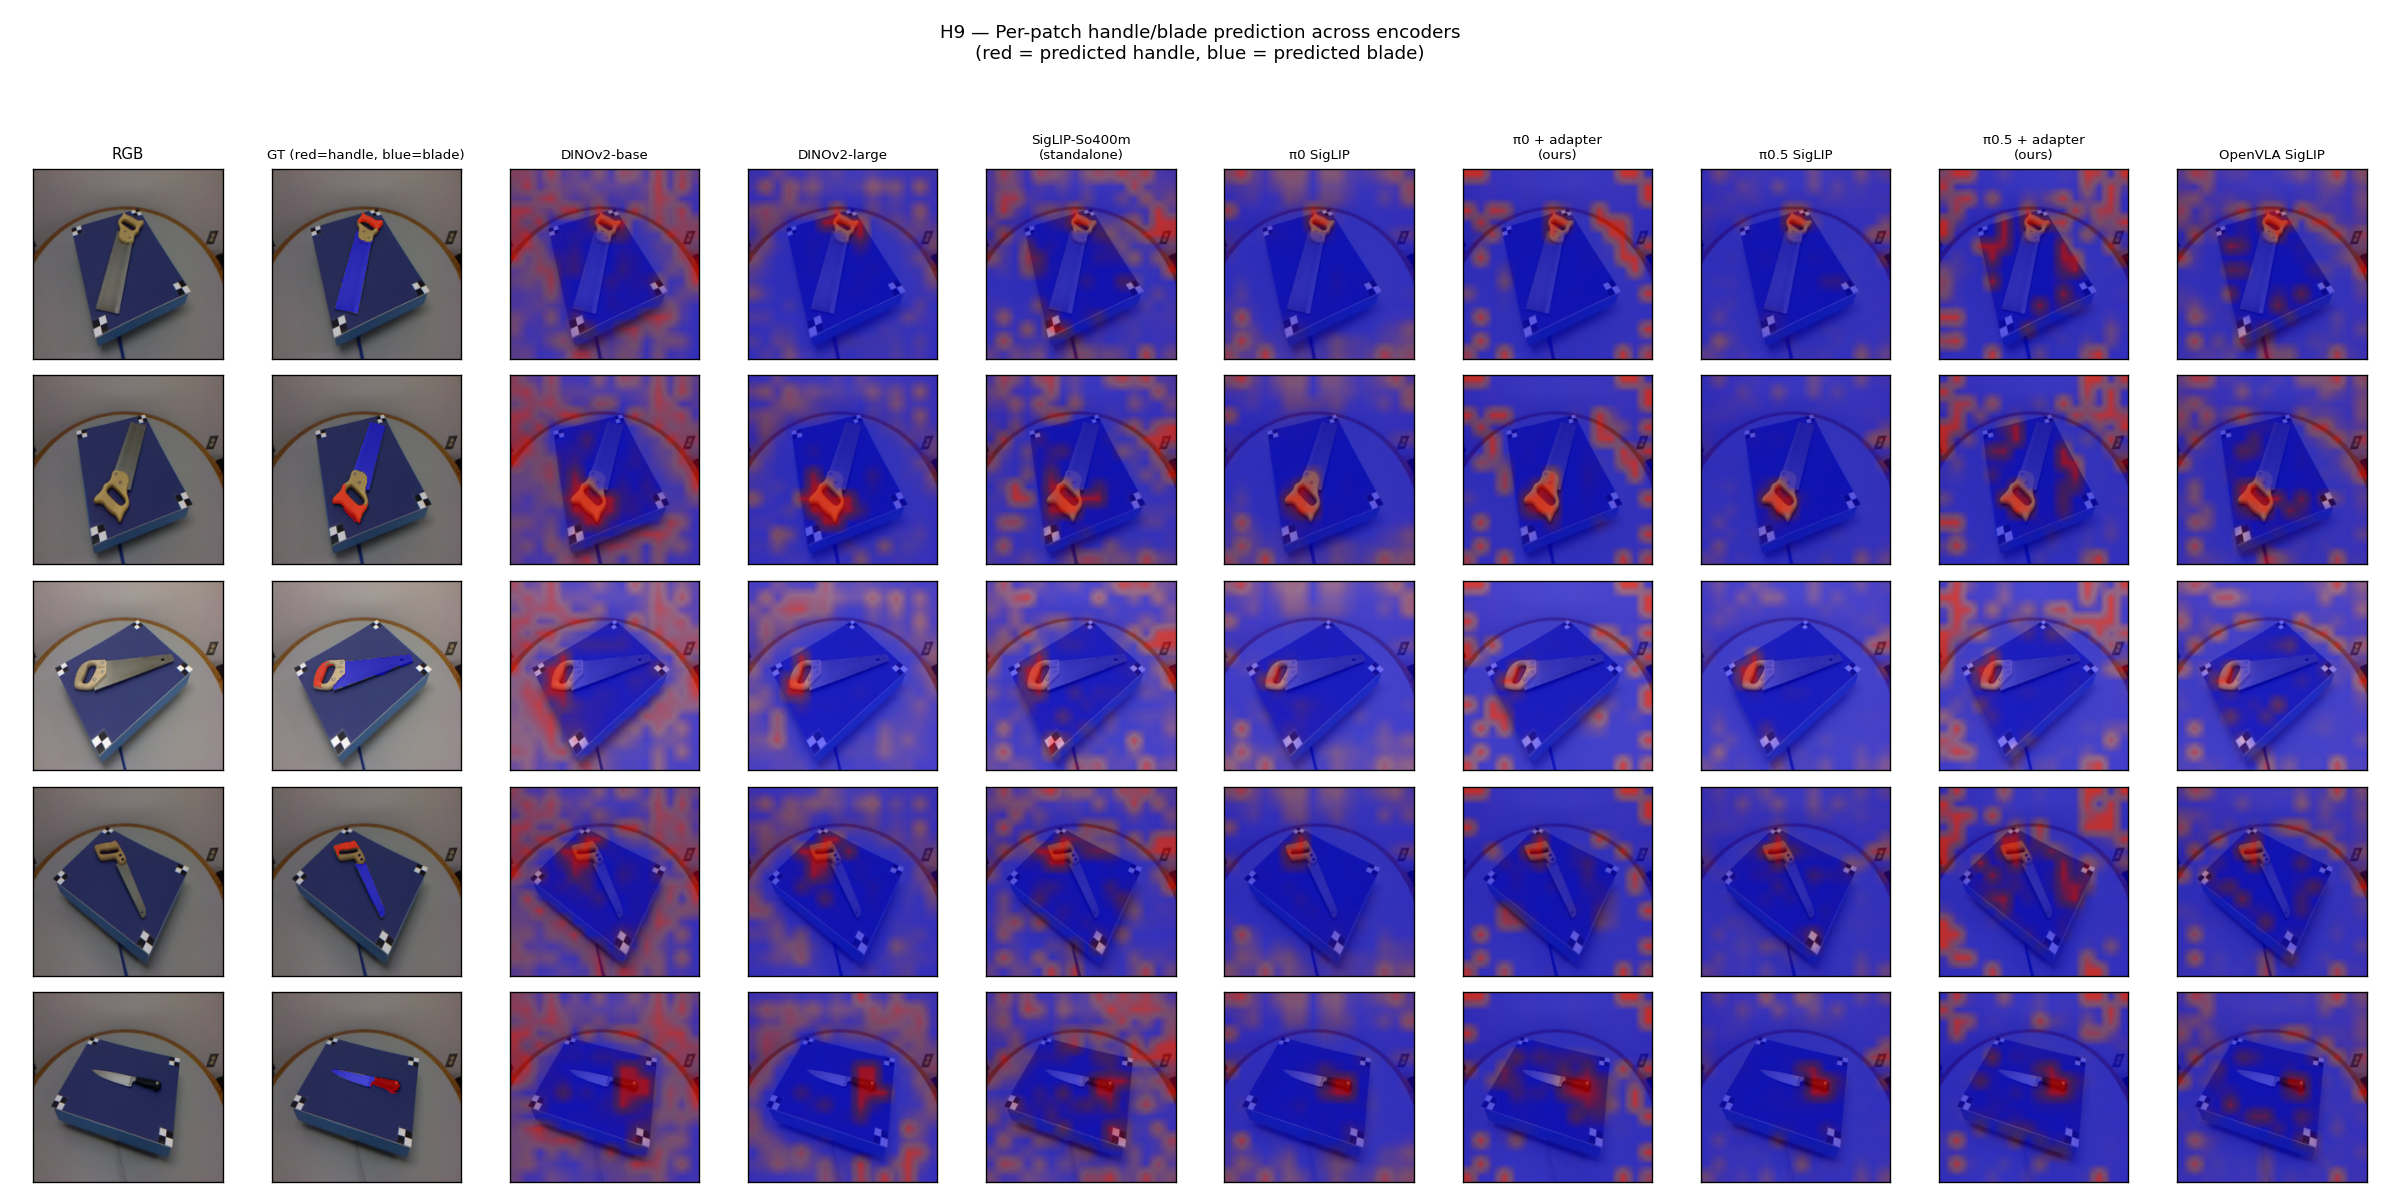
\includegraphics[width=\linewidth]{figures/h9_qualitative.png}
\caption{Held-out UMD test images. Red = predicted handle
(\texttt{grasp}); blue = predicted blade (\texttt{cut}). Across all
seven encoders, including the VLAs that ``lost'' \texttt{cut} under
H2 multi-class probing, predicted blade regions land on the actual
cutting edge.}
\label{fig:qual}
\end{figure}

Figure~\ref{fig:qual} shows per-patch handle/blade probability maps for
all seven encoders on held-out UMD knife and shears images. Despite the
27\,pp multi-class deficit, the VLA encoders' binary handle/blade
predictions land on the correct sub-regions. The qualitative picture
matches the complexity-spectrum quantitative result.

\subsection{Companion experiment: ManiSkill3 PickCube}

\begin{figure}[t]
\centering
\begin{subfigure}{0.49\linewidth}
\centering
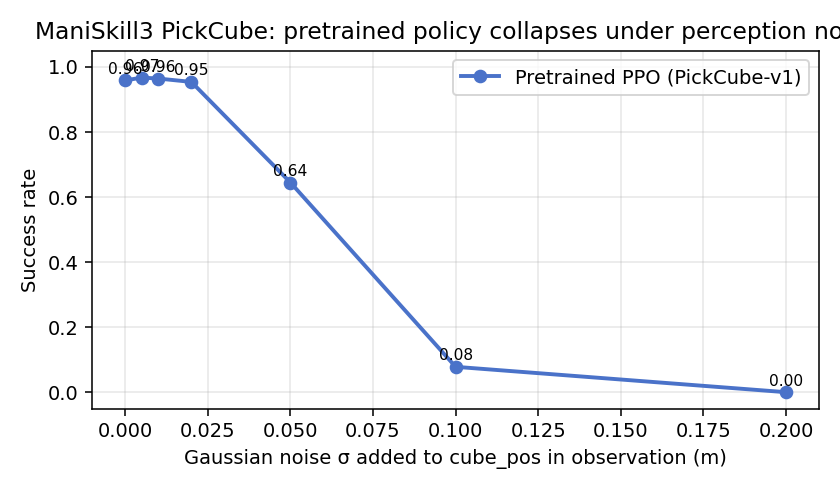
\includegraphics[width=\linewidth]{figures/h6_robustness.png}
\caption{Pretrained PPO success vs.\ Gaussian noise on the cube\_pos
state slice. 10\,cm noise drops success from 0.96 to 0.22.}
\label{fig:h6_robustness}
\end{subfigure}\hfill
\begin{subfigure}{0.49\linewidth}
\centering
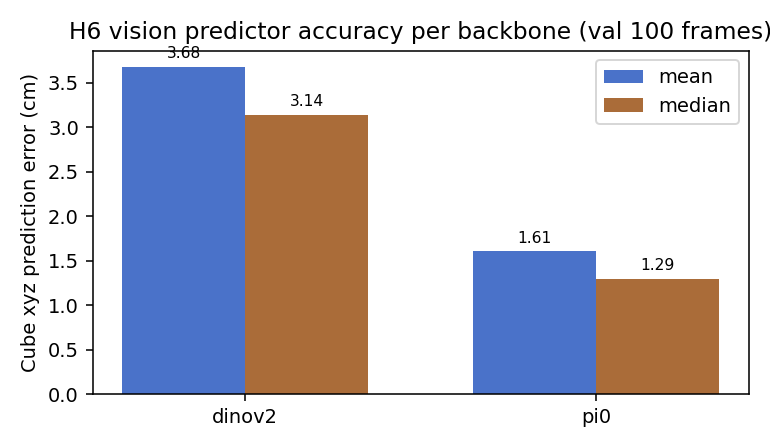
\includegraphics[width=\linewidth]{figures/h6_predictor.png}
\caption{Cube-position regression error from frozen patch features.
$\pi_0$ SigLIP wins on this geometric (\texttt{contain}-class) task.}
\label{fig:h6_predictor}
\end{subfigure}
\caption{ManiSkill3 PickCube companion experiment. (a) state-conditioned
PPO is fragile to perception error. (b) $\pi_0$'s vision tower predicts
cube position 2$\times$ better than DINOv2-base on this geometric task,
exactly as the H2 per-class structure (\texttt{contain} preserved) predicts.}
\label{fig:h6}
\end{figure}

We ran a downstream perception experiment on ManiSkill3
\cite{tao2024maniskill3} PickCube --- a \texttt{contain}-class
manipulation task --- using each VLA's frozen vision tower as a feature
extractor for cube-position regression
(Figure~\ref{fig:h6}).
The pretrained ManiSkill3 PPO checkpoint solves PickCube at 96\%
success on clean state but collapses to 22\% under 10\,cm Gaussian
noise on the cube-position observation slice
(Figure~\ref{fig:h6_robustness}). State-conditioned policies are
extremely fragile to perception error.

We then trained Ridge regressors over mean-pooled patch features that
map RGB to 3D cube xyz, on 400 rendered frames per encoder.
$\pi_0$ SigLIP achieves 1.61\,cm mean L2 error vs.\ DINOv2-base's
3.68\,cm (Figure~\ref{fig:h6_predictor}). Two-fold improvement.

This is a clean downstream confirmation of the H2 per-class structure:
$\pi_0$ preserved \texttt{contain}-class affordance, and PickCube
cube-position is a \texttt{contain}-class quantity, so $\pi_0$'s vision
tower outperforms uninstructed DINOv2 on this task. The per-class
probing scores correctly predicted the per-task downstream winner.

% =====================================================================
\section{Discussion}
\label{sec:discussion}

\paragraph{What the work establishes.}
VLA fine-tuning corrupts affordance representations in a structured,
recoverable way. The corruption is class-asymmetric (\texttt{cut}
destroyed, \texttt{contain} preserved), family-general (PaliGemma and
Prismatic-Llama show the same pattern), recipe-dependent ($\pi_{0.5}$
partially recovers cut), mechanistically localised (final-layer
rotation, with class-selective drift correlated to per-class IoU drop),
and recoverable with a 297\,K-parameter adapter on frozen features. On
the geometric subset of downstream tasks, post-VLA encoders actually
outperform uninstructed baselines.

\paragraph{What surprised us.}
The headline finding from H2 --- ``$\pi_0$ catastrophically loses cut
affordance'' --- did not survive the complexity-spectrum analysis. We
expected the 27\,pp deficit to manifest on any cut-related task; in
practice it collapses on every binary part-discrimination formulation.
This is a significant nuancing of the existing affordance-probing
literature: the standard 5-class IoU metric over-reports the deficit
relative to the perception sub-problem manipulation actually solves.

\paragraph{Why $\pi_0$ rotates the final layer so heavily.}
$\pi_0$'s flow-matching action head reads action tokens that
cross-attend with the SigLIP final-layer outputs. The encoder is
pressured to lay out the final-token directions to support action
prediction; our final-layer CKA of 0.023 indicates a near-orthogonal
rotation. $\pi_{0.5}$'s improved recipe spreads this pressure across
middle layers (final CKA = 0.36), preserving more of the original
geometry overall but with less geometric specialisation in the late
features. OpenVLA's autoregressive action token requires less rotation
of the encoder than $\pi_0$'s continuous-action head.

\paragraph{Why the loss is class-asymmetric.}
\texttt{cut} requires distinguishing handle from blade --- an
edge-orientation cue. We hypothesise that $\pi_0$'s training corpus
contains few cutting primitives, so the encoder has no incentive to
preserve edge-orientation directions in linearly readable form.
\texttt{contain} and \texttt{scoop} require coarser geometric cues
(concavity, opening) that benefit pick-and-place primitives, which
dominate $\pi_0$'s training data.

% =====================================================================
\section{Limitations and Failure Cases}
\label{sec:limitations}

\paragraph{Single dataset.}
All probing claims are on UMD Part Affordance. Cross-dataset validation
on AGD20K \cite{luo2022agd20k}, IIT-AFF, or 3D AffordanceNet was in
scope but not completed.

\paragraph{No closed-loop manipulation evaluation.}
We did not plug the recovered (adapter) features into a real policy and
measure success rate. The natural follow-up --- LIBERO $\times$ $\pi_0$
per-task success-rate prediction from per-class probe scores ---
requires $\geq 24$\,GB VRAM for $\pi_0$ inference; we had 8\,GB local.

\paragraph{Adapter does not transfer.}
On H10b multi-tool composites, $\pi_0$+adapter drops to 0.85 balanced
accuracy versus raw $\pi_0$'s 0.93. The adapter is dataset-specific.
We report this as a documented failure mode rather than a fix.

\paragraph{Mechanism correlation has low n.}
$n = 5$ affordance classes per VLA. Significant for two of three VLAs
but underpowered. A wider taxonomy would harden the result.

\paragraph{Recovery via state override fails.}
We attempted to use the cube-position predictor's output to override the
PPO policy's state observation under noise. Oracle override gives 100\%
success at all noise levels; vision-predicted override stays flat at
$\sim$7\%, \emph{worse} than the noisy baseline. Diagnostic: ManiSkill3
encodes cube position redundantly across multiple state slices; partial
override creates contradictory signals. We document this as a real
intervention-design lesson: to inject affordance into a state-conditioned
policy, the affordance signal must be consistent with all task-relevant
state slices, or the policy must be retrained from pixels-only.

% =====================================================================
\section{Future Work}
\label{sec:future}

The natural extensions of this work cluster around closing the loop
from per-class probing to per-task manipulation success.

\paragraph{LIBERO $\times$ $\pi_0$ per-task crossover.}
Group LIBERO's 130 tasks by primary affordance class, run $\pi_0$
zero-shot, measure per-class success rate, correlate with H2 per-class
IoU. If correlation is significant, the chain ``encoder probing $\to$
policy success'' closes. Compute: $\sim$40 GPU-hours on an A100.

\paragraph{Adapter on a real policy.}
Train a vision-only manipulation policy from scratch on a part-aware
task (knife-handle grasping in ManiSkill3 PickSingleYCB) with three
perception heads: DINOv2, $\pi_0$ raw, $\pi_0$+adapter. Measure success
rate; predict the ranking from the H2 per-class structure.

\paragraph{Cross-dataset validation.}
Run the same probing protocol on AGD20K (36 affordance classes, 20K
images) and IIT-AFF. If the class-asymmetric pattern persists, the
finding generalises beyond UMD.

\paragraph{More VLA families.}
Extend to Octo \cite{octo2024}, RT-2 \cite{rt22023}, and Cosmos-Policy
\cite{cosmospolicy2025}. Three families is the minimum for a
``recipe-independent'' claim; five would harden it.

% =====================================================================
\section{Conclusion}
\label{sec:conclusion}

We measured the per-class structure of affordance loss inside three
deployed vision-language-action encoders. The loss is class-asymmetric
($\texttt{cut} -27$\,pp, $\texttt{contain} -1$\,pp on $\pi_0$),
generalises across two VLA families, is mechanistically localised
(final-layer rotation, with class-selective drift correlated to
per-class IoU drop at $\rho = 0.90$ on $\pi_0$), and is recoverable
with a 297\,K-parameter adapter that closes 82\% of the cut-class gap
on frozen features. However, on the binary part-discrimination
formulations downstream manipulation pipelines actually use, the
apparent 27\,pp deficit collapses to $\leq 3$\,pp --- the standard
multi-class probe overstates the encoder deficit relative to the
perception sub-problem manipulation actually solves.

% =====================================================================
\section*{Code and reproducibility}

All code, intermediate results, slides, and figures are available at
\url{https://github.com/nitik1998/PAVE} under MIT license. Every
result in this paper is reproducible from the public repository on a
single 8\,GB consumer GPU.

% =====================================================================
\bibliographystyle{plain}
\bibliography{refs}

\end{document}
